VISOR is not officially supported by the KR1410 and there is no direct integration of the camera available.
However, Kassow robots provides support to build own software through CBun development.
The CBun (Capability Bundle) represents a modular framework within the KR software system,
which encapsulates functionalities and provides the
access to its predefined \hyperref[acro:API]{API}. \cite{Cbun}


\begin{figure}[h]
    \centering
    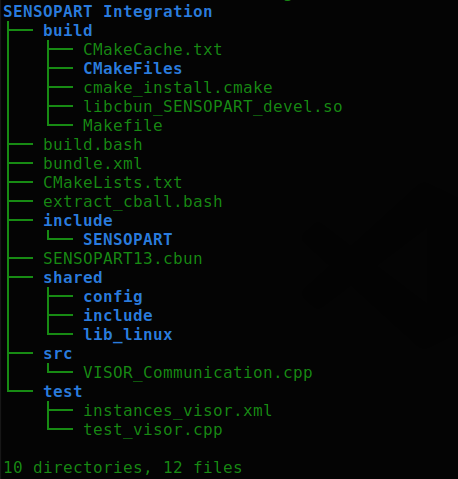
\includegraphics[width=0.5\textwidth]{figures/sensopart-development.png}
    \caption{CBun Project Setup for SENSOPART Integration in KR}
    \label{fig:sensopart-development}
\end{figure}

The CBun SDK is the Software Development Kit that provides all essential tools for CBun development. In order to develop CBuns with the CBun SDK you need a so called CBun build environment which is based on a certainly
configured Ubuntu 18.04 Linux OS with a special set of software packages (such as Kassow Robots APIs).

The recommended CBun development environment setup is based on the Visual Studio Code Dev Containers extension. With this you can develop your CBun in Visual Studio Code on Windows, MacOS or Linux without the need for complicated build environment configuration.
In order to setup your CBun build environment please follow the Build Environment Setup.

Learn the basics of CBun project structure with the Introduction.

Follow the Device, Command or Application (CBunX) guide to define your own CBun element.

Use the Code Snippets to implement the element's behaviour.

To setup the communication between the KR1410 and the VISOR vison sensor, customme